\documentclass[12pt,a4paper]{article}
\usepackage[utf8]{vietnam}
\usepackage{graphicx}
\usepackage{geometry}
\usepackage{array}
\usepackage{hyperref}
\usepackage{titlesec}
\usepackage{multirow}
\usepackage[table]{xcolor}
\usepackage{listings} % Để hiển thị code đẹp hơn
\usepackage{float}

\geometry{a4paper, margin=2cm}

% Cấu hình hiển thị code
\lstset{
  basicstyle=\ttfamily\small,
  breaklines=true,
  frame=single,
  backgroundcolor=\color{gray!10},
  keywordstyle=\color{blue},
  commentstyle=\color{green!50!black},
  stringstyle=\color{red}
}

\begin{document}

% --- TRANG BÌA (Giữ nguyên như bạn đã có) ---
\begin{center}
    \textbf{TRƯỜNG ĐẠI HỌC CÔNG NGHỆ THÔNG TIN}\\
    \vspace{1cm}
    
\includegraphics[width=4cm]{logo-uit.png} % Thay bằng tên file logo của bạn
    \vspace{1cm}
    
    \textbf{\Large BÁO CÁO THỰC HÀNH 01}\\
    \vspace{0.5cm}
    \textbf{Dùng Terraform và CloudFormation để quản lý và triển khai hạ tầng AWS}\\
\end{center}

\vspace{0.5cm}
\begin{flushleft}
    \textbf{Môn học: }Công nghệ DevOps và ứng dụng\\
    \textbf{Lớp:} NT548.Q11 \\
\end{flushleft}

\noindent
\begin{minipage}[t]{0.65\textwidth}
    \vspace{0pt}
    \textbf{\underline{THÀNH VIÊN THỰC HIỆN (Nhóm 15):}}
    \vspace{0.5em}
    \begin{tabular}{|c|l|c|}
        \hline
        \textbf{STT} & \textbf{Họ và tên} & \textbf{MSSV} \\ \hline
        1 & Võ Đình Trung & 22521571 \\ \hline
        2 & Trương Phúc Trường & 22521587 \\ \hline
        3 & Lê Văn Vũ & 23521809 \\ \hline
    \end{tabular}
\end{minipage}%
\hfill
\begin{minipage}[t]{0.3\textwidth}
    \vspace{0pt} 
    \centering
    \begin{tabular}{|>{\centering\arraybackslash}p{4cm}|}
        \hline
        \textbf{Điểm tự đánh giá} \\ \hline
        \vspace{0.75cm} 
        \textbf{\Large 9.5} 
        \vspace{0.75cm} \\ \hline
    \end{tabular}
\end{minipage}

\vspace{1cm}
\begin{flushleft}
\textbf{\underline{ĐÁNH GIÁ KHÁC:}}
\begin{table}[H]
    \begin{tabular}{|p{5cm}|p{10cm}|}
        \hline
        \textbf{Tổng thời gian thực hiện} & 48 giờ \\ \hline
        \textbf{Phân chia công việc} & Trung: Cấu hình và triển khai, sửa lỗi sơ bộ Terraform network (VPC/NAT)\& EC2, hỗ trợ viết báo cáo  \&  Security Groups; Trường: Chạy sau cùng và lấy kết quả viết báo cáo; Vũ: Chạy kiểm thử và sửa lỗi còn lại. \\ \hline
        \multirow{2}{*}{\textbf{Ý kiến (nếu có)}} & + Khó khăn: Việc quản lý địa chỉ IP gặp nhiều trở ngại do Public IP của EC2 thay đổi sau mỗi lần terraform destroy/apply, làm mất kết nối SSH và phải cập nhật lại file cấu hình thủ công\\ \cline{2-2}
         & + Giải pháp: Nhóm đề nghị sử dụng Elastic IP (EIP) cho Bastion và NAT Gateway để cố định điểm truy cập ở lần cấu hình sau. Đồng thời, kiến nghị sử dụng thêm Ansible hoặc Dynamic DNS trong các bài Lab sau và đồ án để tự động hóa quy trình. \\ \hline
    \end{tabular}
\end{table}
\end{flushleft}

\newpage

% --- PHẦN B: BÁO CÁO CHI TIẾT ---
\section*{B. BÁO CÁO CHI TIẾT} 

\noindent
\textbf{GitHub Repository:} \href{https://github.com/votrung654/EShelf}{https://github.com/votrung654/EShelf}

\section*{Tổng quan: Thiết lập môi trường}
Trước khi triển khai các dịch vụ cụ thể, nhóm đã thiết lập cấu trúc dự án Terraform theo mô hình modules để đảm bảo tính tái sử dụng và quản lý mã nguồn hiệu quả:
\begin{itemize}
    \item \textbf{Provider:} AWS (Region: \texttt{ap-southeast-2}).
    \item \textbf{State Management:} Lưu trữ local (đã triển khai mở rộng lên S3 nhưng chưa hoàn thiện).
    \item \textbf{Cấu trúc thư mục:} Phân tách rõ ràng \texttt{terraform/modules/vpc}, \texttt{terraform/modules/ec2}, \texttt{terraform/modules/security\_groups}.
\end{itemize}
\begin{figure}[H]
    \centering
    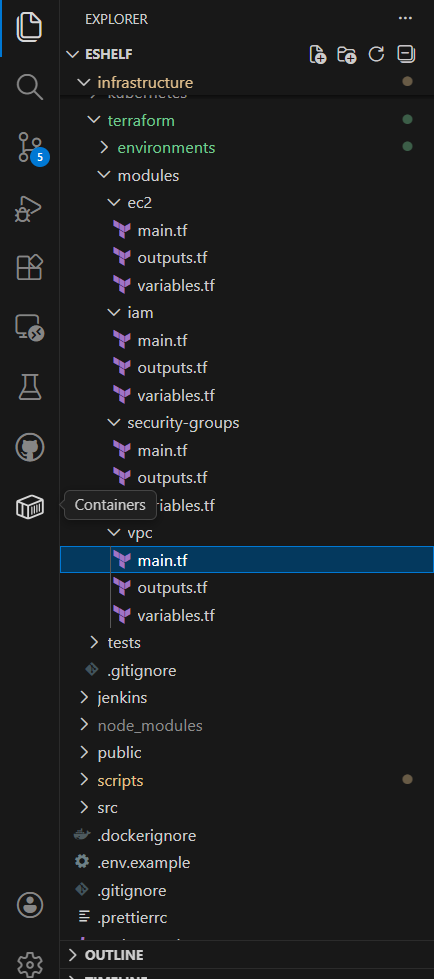
\includegraphics[width=0.4\textwidth]{img/image_0.png} 
    \caption{Cấu trúc chia theo modules}
\end{figure}
% === CÂU 1: VPC ===
\section*{Câu 1: Triển khai Virtual Private Cloud (VPC)}
\subsection*{1.1 Cấu hình và thiết lập}
Dựa trên yêu cầu bài tập, nhóm đã tạo một VPC đóng vai trò là mạng lõi cho toàn bộ hệ thống eShelf:

\begin{itemize}
    % \item \textbf{CIDR Block:} \texttt{10.0.0.0/16} (Cung cấp 65,536 địa chỉ IP).
    \item \textbf{Phân chia Subnets:}
        \begin{itemize}
            \item \textbf{Public Subnets:} Chứa các tài nguyên cần giao tiếp trực tiếp với Internet (Bastion Host).
            \item \textbf{Private Subnets:} Chứa các tài nguyên cần bảo mật (K3s Master, Workers) sử dụng NAT Gateway để kết nối ra ngoài.
        \end{itemize}
    \item \textbf{Internet Gateway (IGW):} Đã gắn vào VPC để cung cấp đường ra Internet cho Public Subnet.
\end{itemize}
\begin{figure}[H]
    \centering
    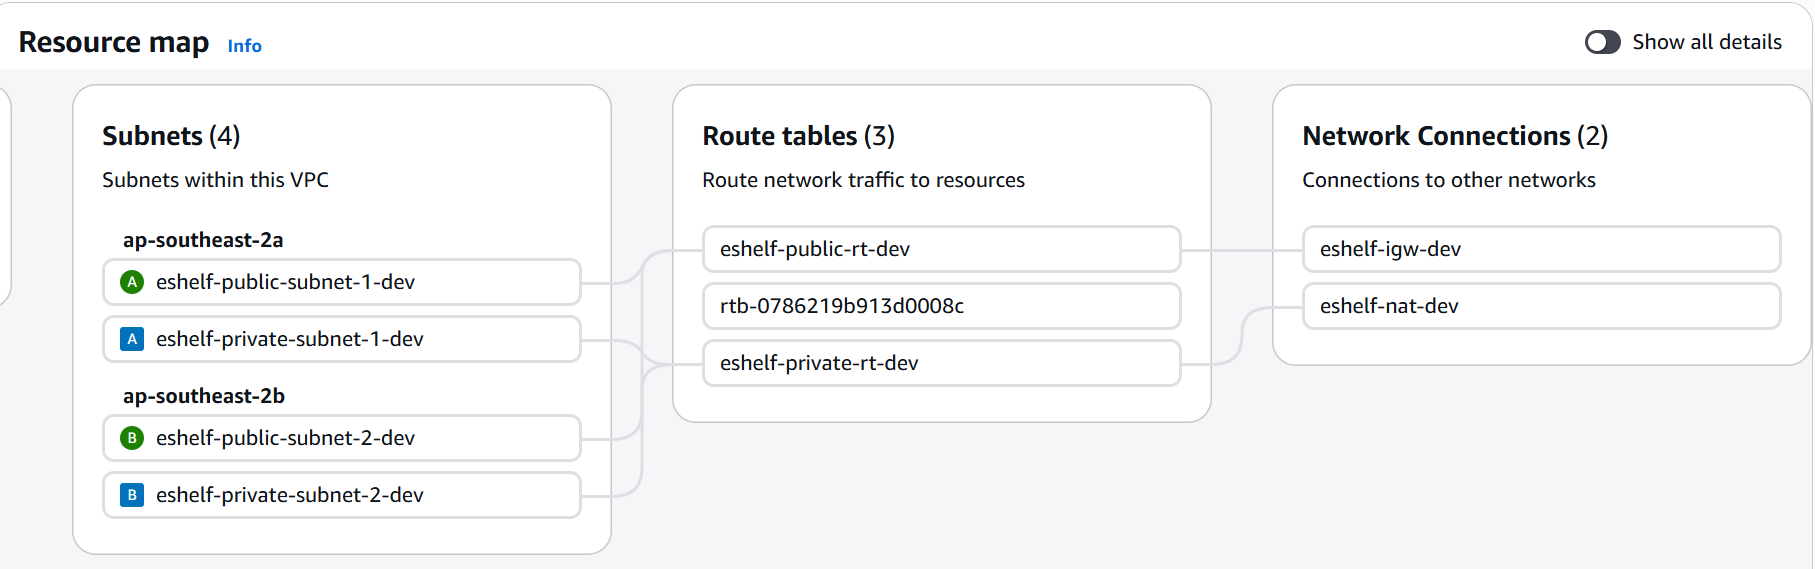
\includegraphics[width=0.9\textwidth]{img/vpc_resource_map.png} 
    \caption{Sơ đồ VPC Resource Map trên AWS Console}
\end{figure}
% --- PHẦN BỔ SUNG MỚI: DEFAULT SECURITY GROUP ---
% \subsection*{Cấu hình Default Security Group}
Nhóm đã cấu hình \textbf{Default Security Group} của VPC để kiểm soát các tài nguyên chưa được gán nhóm bảo mật cụ thể:
\begin{itemize}
    \item \textbf{Ingress (Luồng vào):} \texttt{DENY ALL} (Chặn toàn bộ) hoặc chỉ cho phép từ chính nó (Self-reference) để ngăn chặn truy cập trái phép do cấu hình sai sót.
    \item \textbf{Egress (Luồng ra):} Cho phép lưu lượng ra ngoài bình thường để cập nhật hệ thống.
\end{itemize}

% \textit{(Cấu hình này được quản lý thông qua resource \texttt{aws\_default\_security\_group} trong Terraform).}
% \subsection{Hình ảnh minh chứng}

\begin{figure}[H]
    \centering
    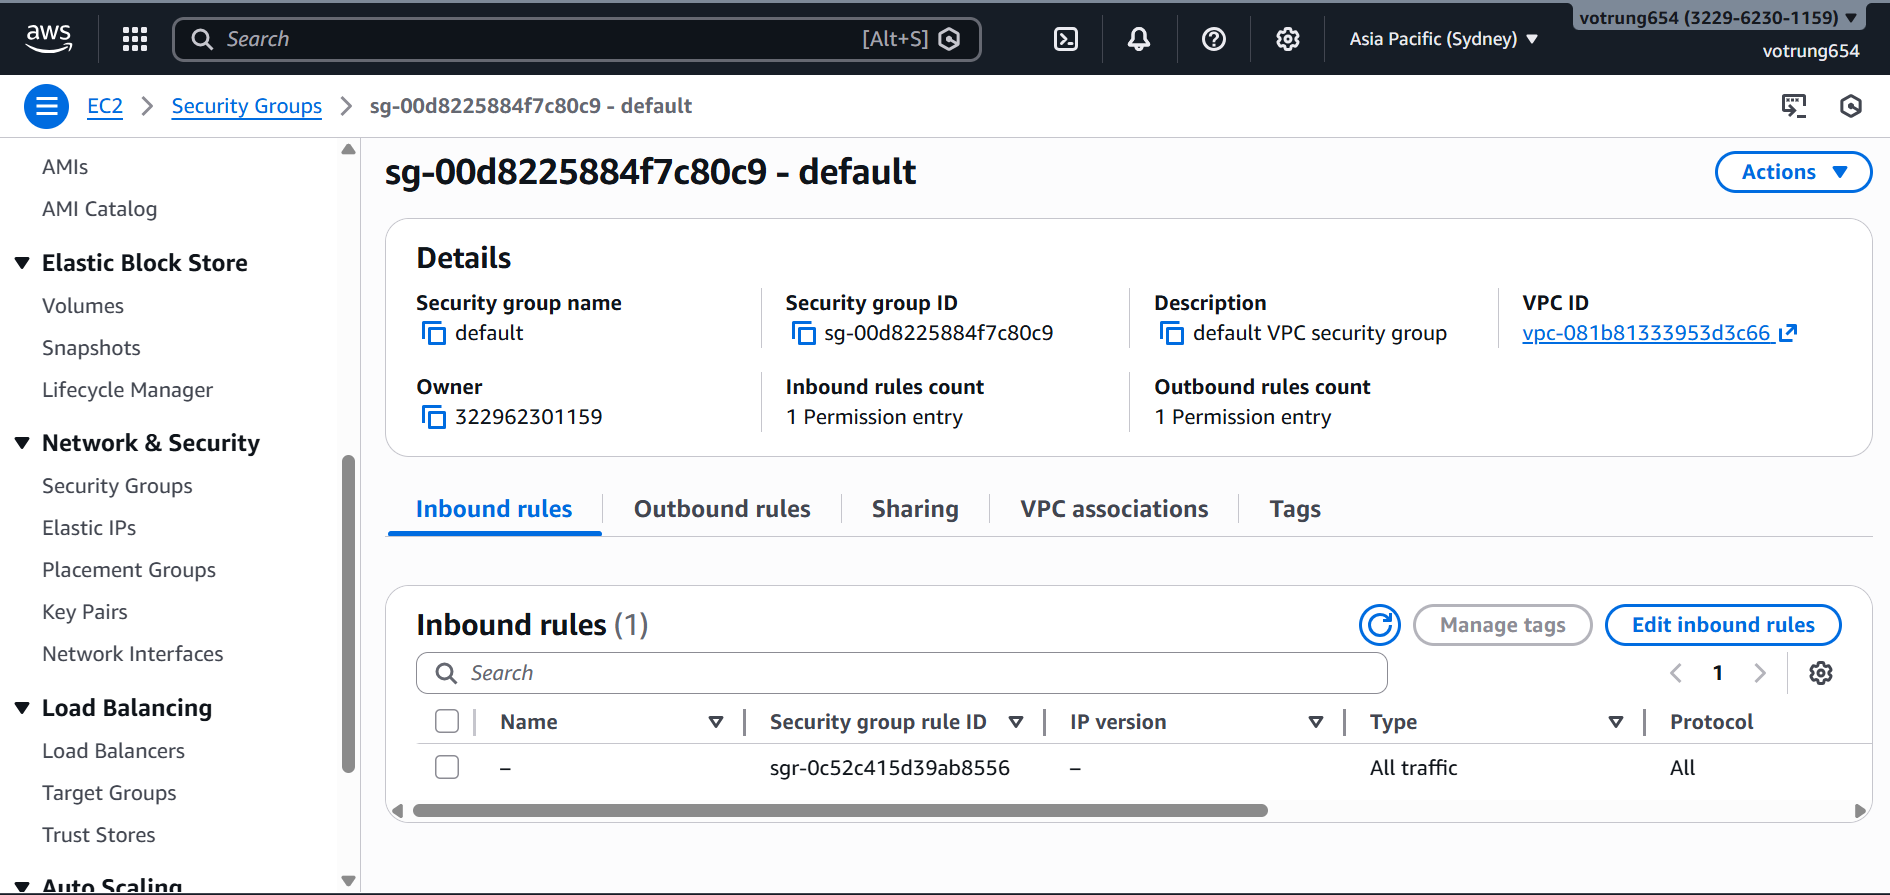
\includegraphics[width=0.9\textwidth]{img/Default_Security_Groups.png} 
    \caption{Default Security Group}
\end{figure}
% -----------------------------------------------------------------
% PHẦN BỔ SUNG: TEST CASES CHO CÂU 1
% -----------------------------------------------------------------
\subsection*{1.2 Kiểm thử kết nối mạng (Network Test Cases)}
Để xác nhận kiến trúc mạng (VPC, Route, NAT) và bảo mật (SG) hoạt động đúng thiết kế, nhóm thực hiện các kịch bản kiểm thử sau:

\begin{table}[H]
    \centering
    \small
    \begin{tabular}{|c|p{4cm}|p{5cm}|p{4cm}|}
        \hline
        \rowcolor{gray!20} \textbf{ID} & \textbf{Mục tiêu kiểm thử} & \textbf{Hành động} & \textbf{Kết quả} \\ \hline
        \textbf{TC1} & \textbf{Public Connectivity:} Kiểm tra IGW và Bastion SG & Từ máy local, SSH vào Public IP của Bastion (\texttt{10.0.1.142}). & Kết nối thành công. \\ \hline
        \textbf{TC2} & \textbf{Private Routing:} Kiểm tra định tuyến nội bộ và Private SG & Từ Bastion, SSH vào Private IP của Master Node (\texttt{10.0.1.123}). & Kết nối thành công (Jump Host hoạt động). \\ \hline
        \textbf{TC3} & \textbf{Outbound Internet:} Kiểm tra NAT Gateway & Từ Master Node, chạy lệnh \texttt{curl -I http://www.google.com}. & Trả về HTTP 200 (Có mạng Internet). \\ \hline
    \end{tabular}
    \caption{Bảng Test Cases kiểm tra hạ tầng mạng}
\end{table}

\subsubsection*{Minh chứng hình ảnh thực tế}

\textbf{1. Minh chứng TC1 \& TC2 (SSH Jump và Kiểm tra thông tin Node):}
Hình ảnh dưới đây minh họa quá trình truy cập phân tầng (SSH Jump) và thông tin chi tiết xác thực vị trí của Bastion Host và Master Node:

% --- ẢNH 1: QUÁ TRÌNH SSH ---
\begin{figure}[H]
    \centering
    % Thay tên file ảnh SSH của bạn vào đây
    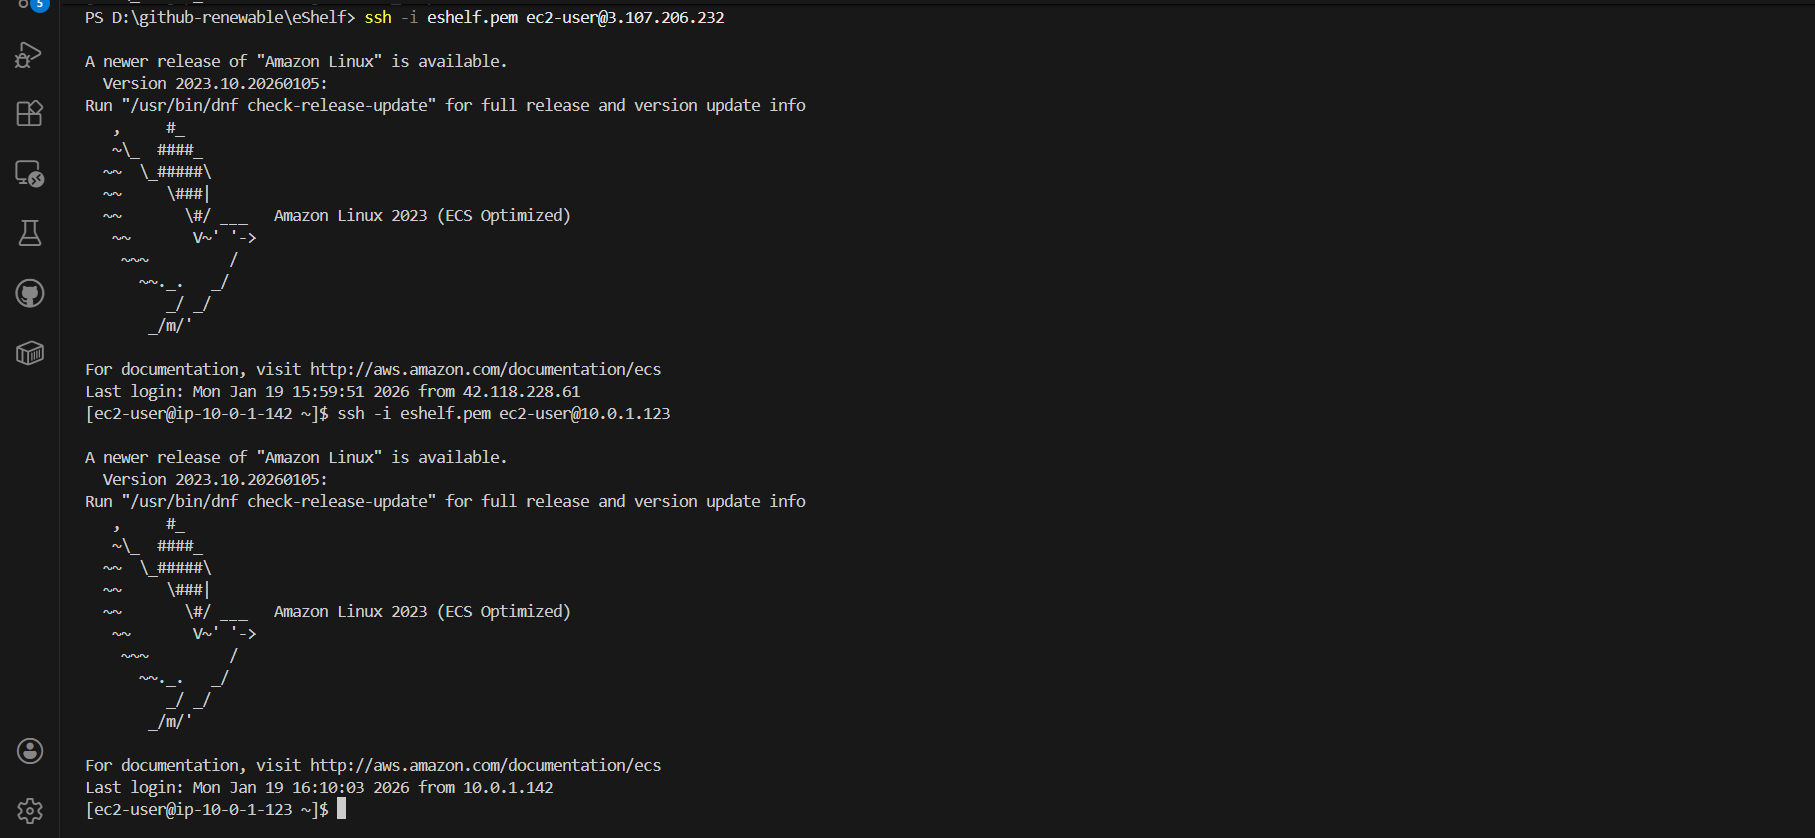
\includegraphics[width=1.0\textwidth]{img/ssh_jump_proof.png}
    \caption{Quá trình SSH từ Local $\rightarrow$ Bastion $\rightarrow$ Master (TC1 \& TC2)}
\end{figure}

% --- ẢNH 2: THÔNG TIN BASTION ---
\begin{figure}[H]
    \centering
    % Thay tên file ảnh thông tin Bastion (ví dụ lệnh: hostnamectl hoặc ip a)
    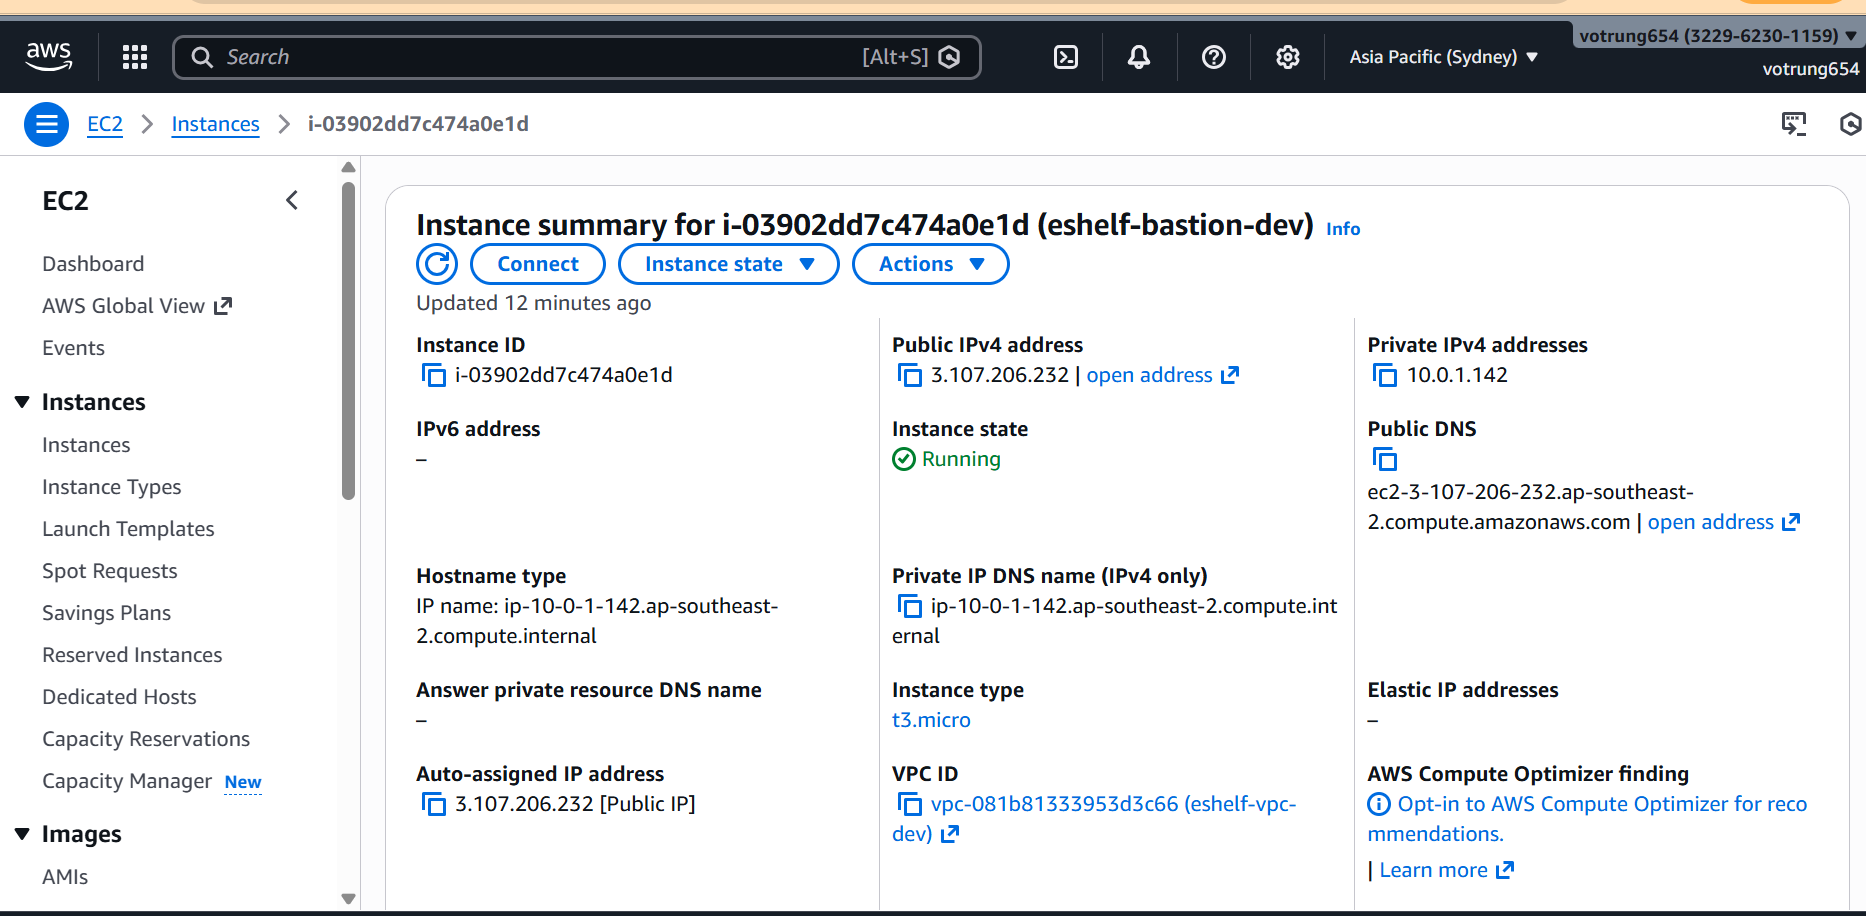
\includegraphics[width=1.0\textwidth]{img/bastion_info.png}
    \caption{Thông tin Bastion Node}
\end{figure}

% --- ẢNH 3: THÔNG TIN MASTER ---
\begin{figure}[H]
    \centering
    % Thay tên file ảnh thông tin Master (ví dụ lệnh: ip a hoặc cat /etc/os-release)
    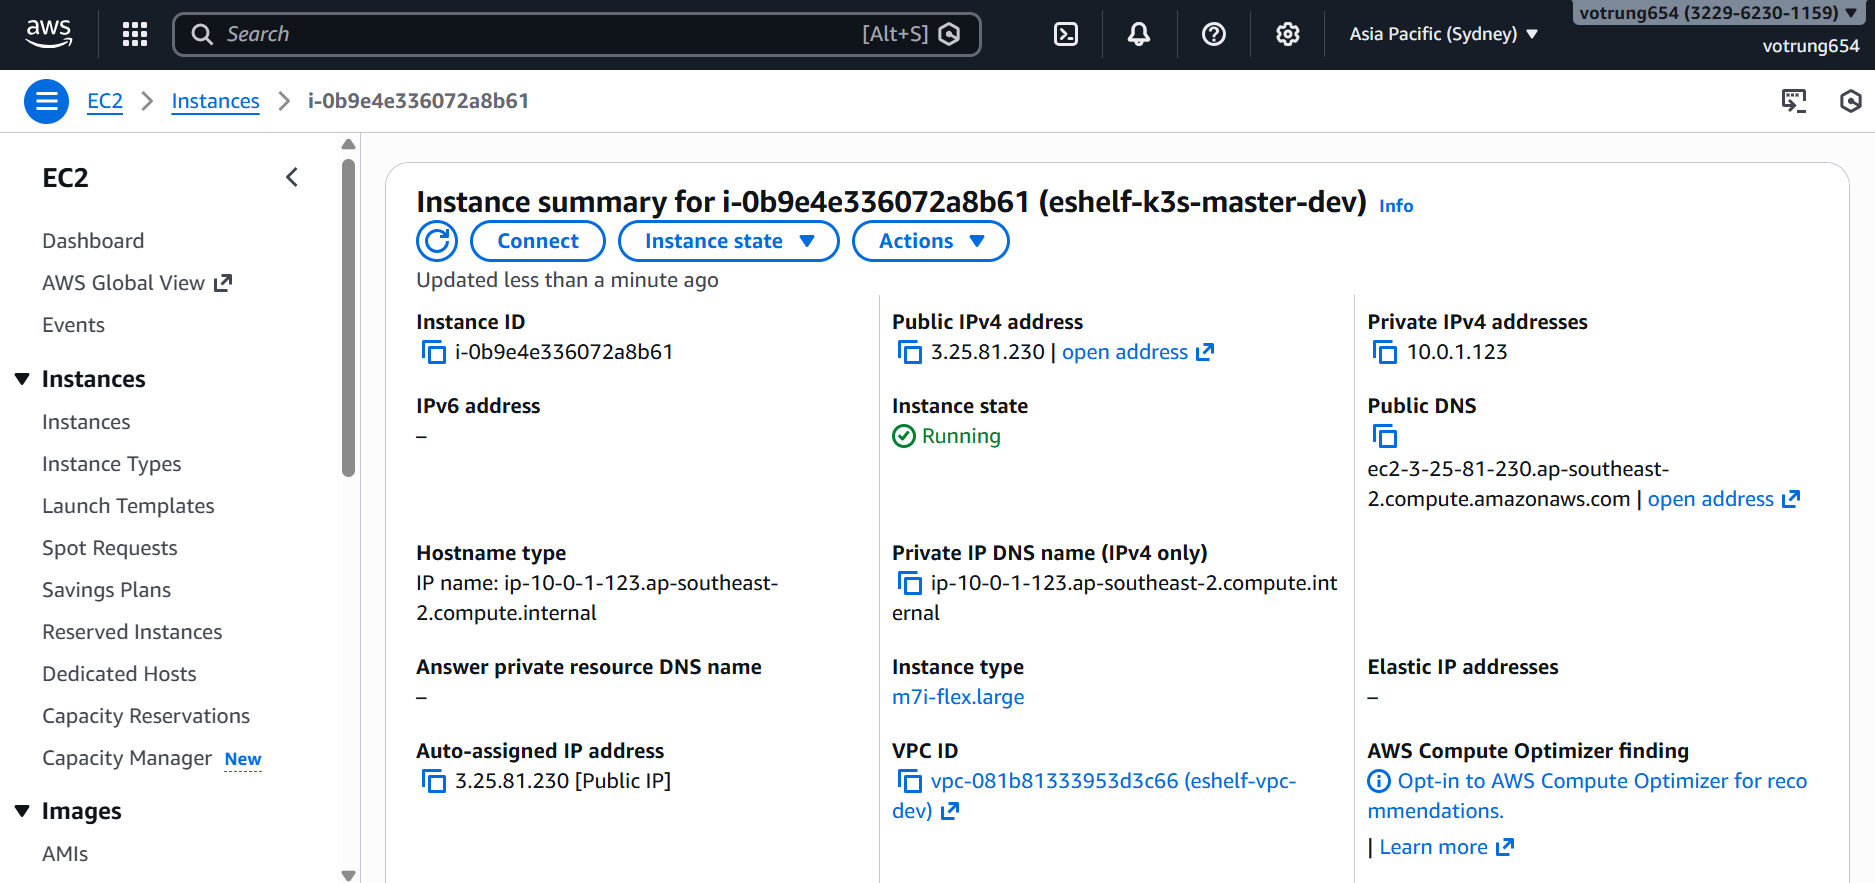
\includegraphics[width=1.0\textwidth]{img/master_info.png}
    \caption{Thông tin Master Node}
\end{figure}

\textbf{2. Minh chứng TC3 (NAT Gateway):}
Hình ảnh kiểm tra kết nối Internet từ máy Master (Private Subnet) thông qua NAT Gateway.
\begin{figure}[H]
    \centering
    % CHỤP ẢNH: Terminal trên máy Master chạy lệnh curl
    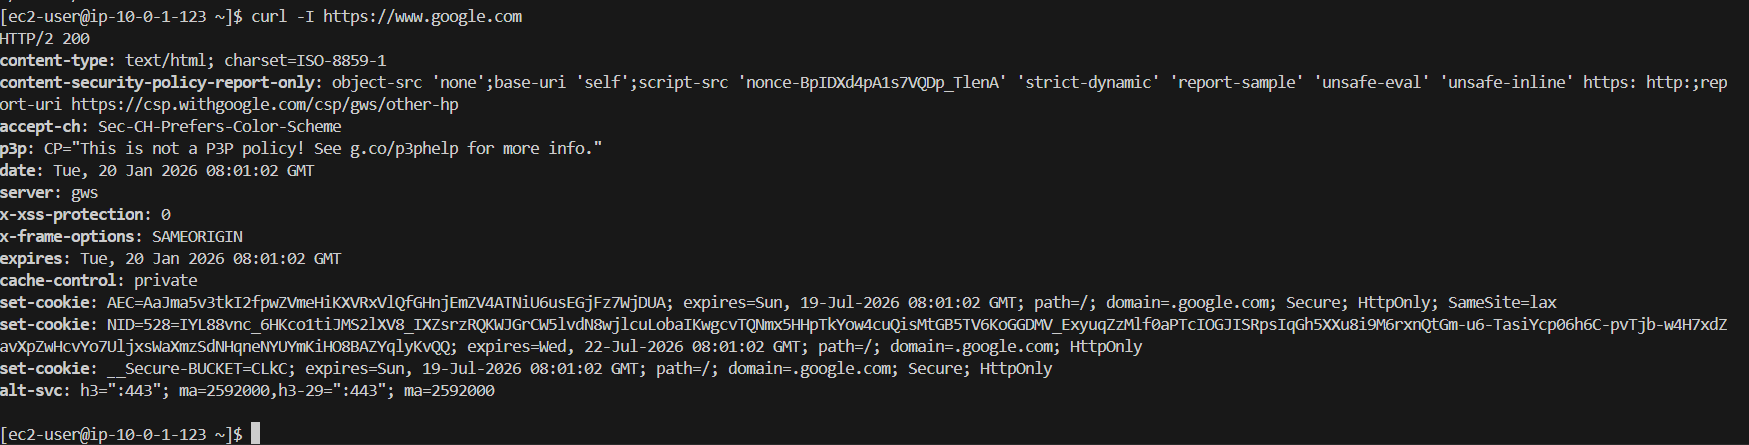
\includegraphics[width=0.9\textwidth]{img/nat.png}
    \caption{Máy Private truy cập Internet thành công qua NAT (TC3)}
\end{figure}

% =================================================================
% CÂU 2: ROUTE TABLES
% =================================================================
\newpage
\section*{Câu 2: Cấu hình Bảng định tuyến (Route Tables)}
\subsection*{2.1 Thiết lập định tuyến}
Để đảm bảo luồng giao thông mạng đi đúng hướng (Public ra IGW, Private qua NAT), nhóm đã cấu hình 2 Route Table riêng biệt:

\begin{itemize}
    \item \textbf{Public Route Table:}
        \begin{itemize}
            \item \textbf{Liên kết:} Gắn với các Public Subnets.
            \item \textbf{Luật định tuyến (Routes):} Destination \texttt{0.0.0.0/0} $\rightarrow$ Target \textbf{Internet Gateway}.
        \end{itemize}
    \item \textbf{Private Route Table:}
        \begin{itemize}
            \item \textbf{Liên kết:} Gắn với các Private Subnets.
            \item \textbf{Luật định tuyến (Routes):} Destination \texttt{0.0.0.0/0} $\rightarrow$ Target \textbf{NAT Gateway}.
        \end{itemize}
\end{itemize}

\begin{figure}[H]
    \centering
    % CHỤP ẢNH: Tab "Routes" của Public Route Table và Private Route Table trên AWS Console
    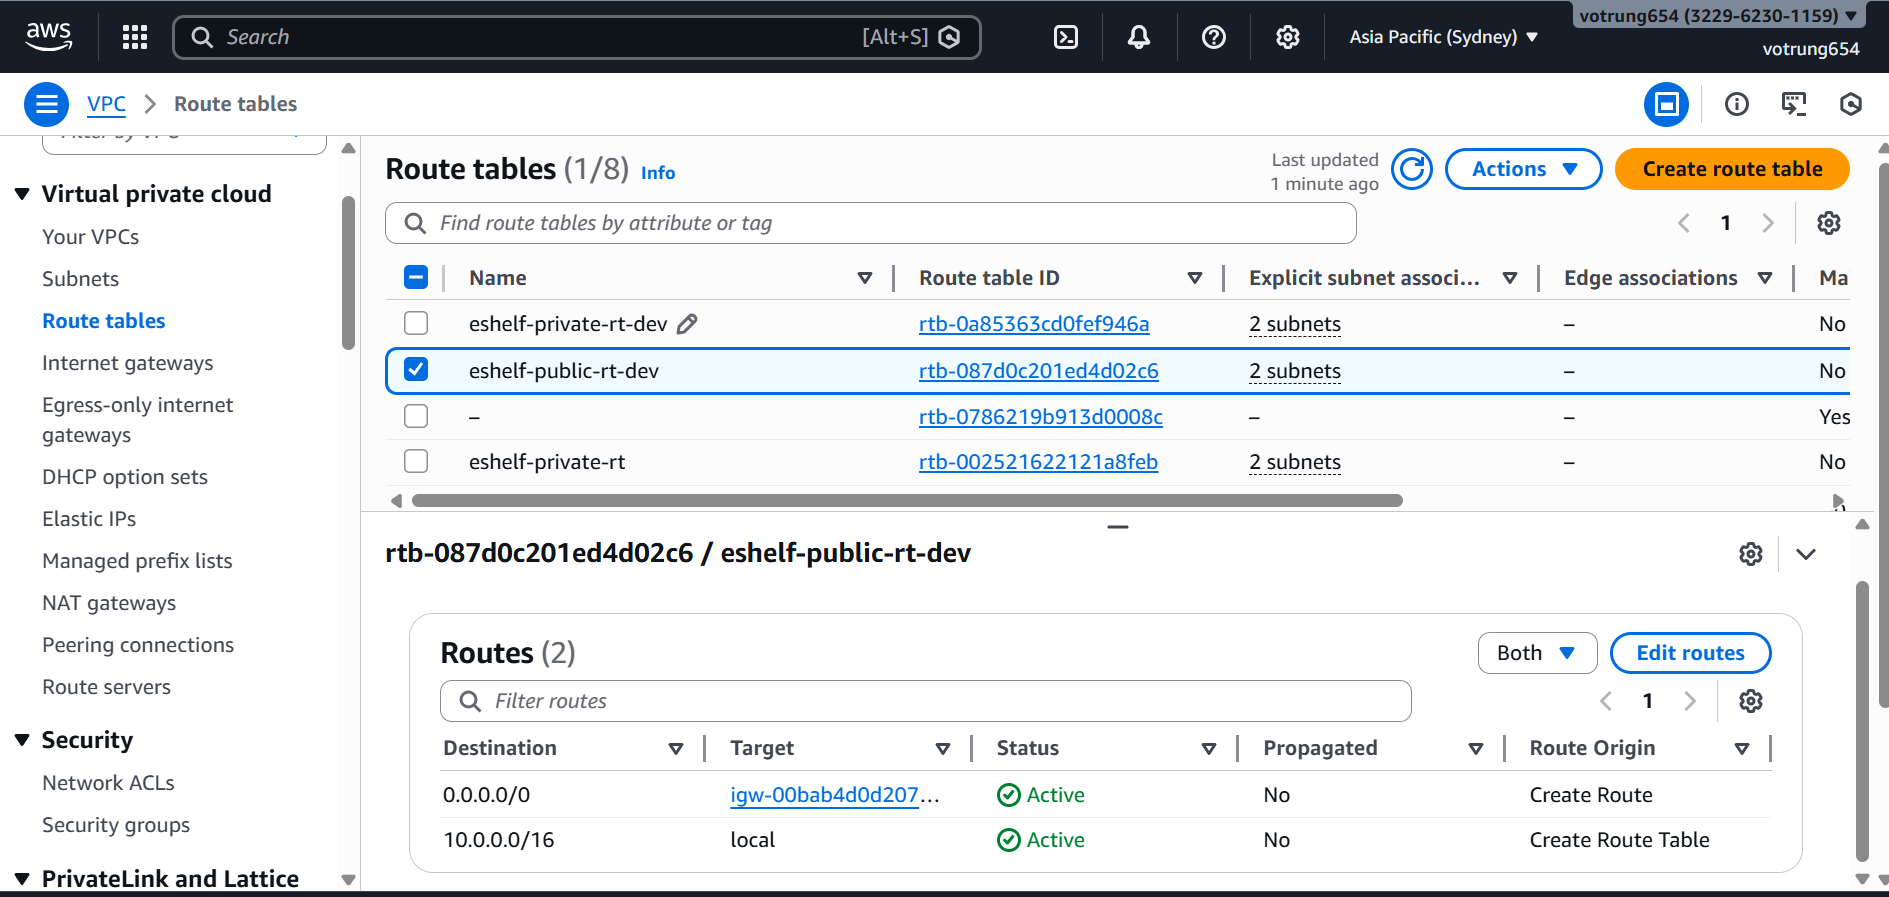
\includegraphics[width=0.7\textwidth]{img/route_tables_igw_config.png} 
    \caption{Cấu hình Routes trỏ về IGW (Public)}
\end{figure}
\begin{figure}[H]
    \centering
    % CHỤP ẢNH: Tab "Routes" của Public Route Table và Private Route Table trên AWS Console
    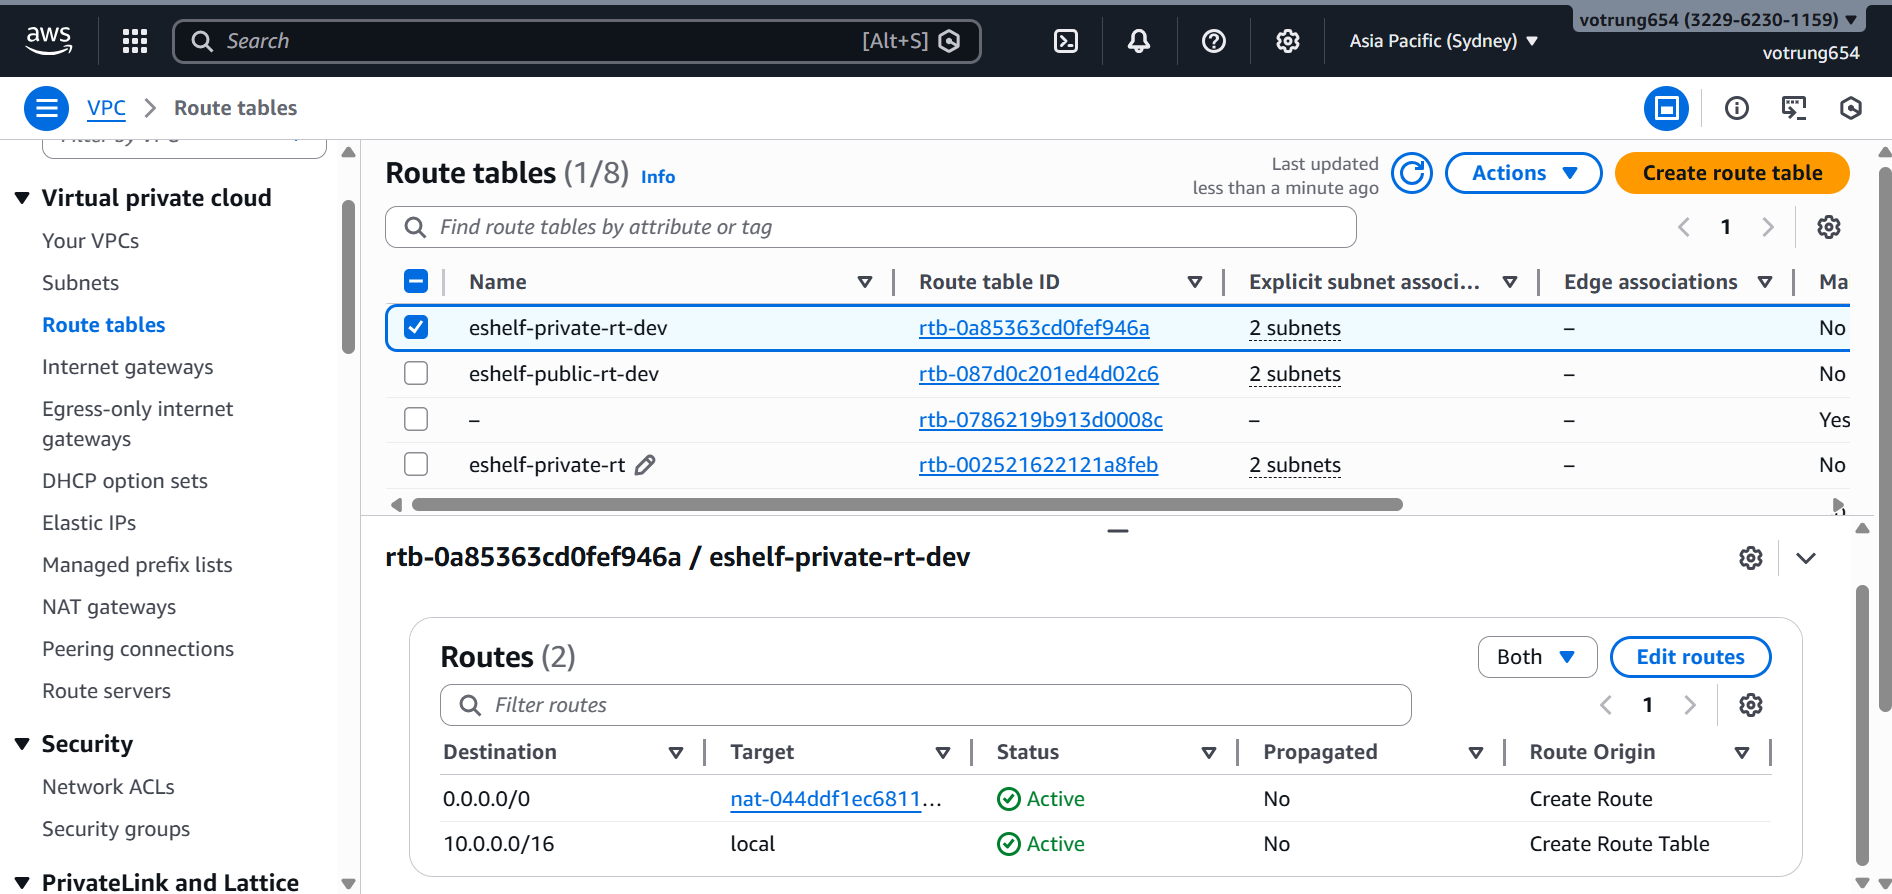
\includegraphics[width=0.7\textwidth]{img/route_tables_nat_config.png} 
    \caption{Cấu hình Routes trỏ về NAT (Private)}
\end{figure}
\subsection*{2.2 Kiểm thử định tuyến (Route Table Test Cases)}
\begin{table}[H]
    \centering
    \small
    \begin{tabular}{|c|p{4cm}|p{5cm}|p{4cm}|}
        \hline
        \rowcolor{gray!20} \textbf{ID} & \textbf{Mục tiêu kiểm thử} & \textbf{Hành động} & \textbf{Kết quả} \\ \hline
        \textbf{TC4} & \textbf{Verify Next Hop:} Kiểm tra đường đi của gói tin từ Private Subnet & Sử dụng lệnh \texttt{traceroute 8.8.8.8} (hoặc tracepath) trên máy Master Node. & Hop đầu tiên hoặc thứ hai phải đi qua địa chỉ IP của NAT Gateway/Network Interface. \\ \hline
    \end{tabular}
    \caption{Kiểm tra định tuyến mạng}
\end{table}
% \subsubsection*{Minh chứng hình ảnh thực tế}
Hình ảnh dưới đây cho thấy gói tin từ máy Master (Private) đã được định tuyến chính xác qua Gateway nội bộ và đi ra ngoài Internet thành công:

\begin{figure}[H]
    \centering
    % DÙNG ẢNH TRACEPATH BẠN VỪA GỬI VÀO ĐÂY
    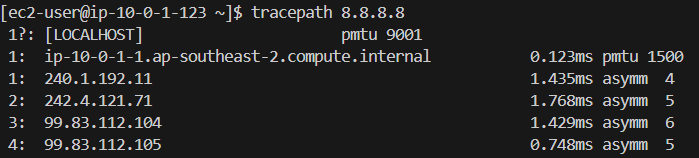
\includegraphics[width=1.0\textwidth]{img/tracepath.png} 
    \caption{Kết quả lệnh tracepath: Xác nhận routing qua NAT thành công (TC4)}
\end{figure}
% =================================================================
% CÂU 3: NAT GATEWAY
% =================================================================
\section*{Câu 3: Triển khai NAT Gateway}
\subsection*{3.1 Cấu hình tài nguyên}
Nhóm triển khai NAT Gateway để cung cấp khả năng truy cập Internet một chiều cho các Private Instances (Master/Worker) nhằm tải các gói tin cài đặt và update hệ thống:
\begin{itemize}
    \item \textbf{Vị trí:} Đặt tại Public Subnet (để có thể giao tiếp với IGW).
    \item \textbf{Elastic IP (EIP):} Đã gán 1 địa chỉ IP tĩnh cố định cho NAT Gateway để đảm bảo IP nguồn không thay đổi khi ra Internet.
\end{itemize}

\begin{figure}[H]
    \centering
    % CHỤP ẢNH: Màn hình chi tiết NAT Gateway trên AWS Console (Hiện trạng thái Available)
    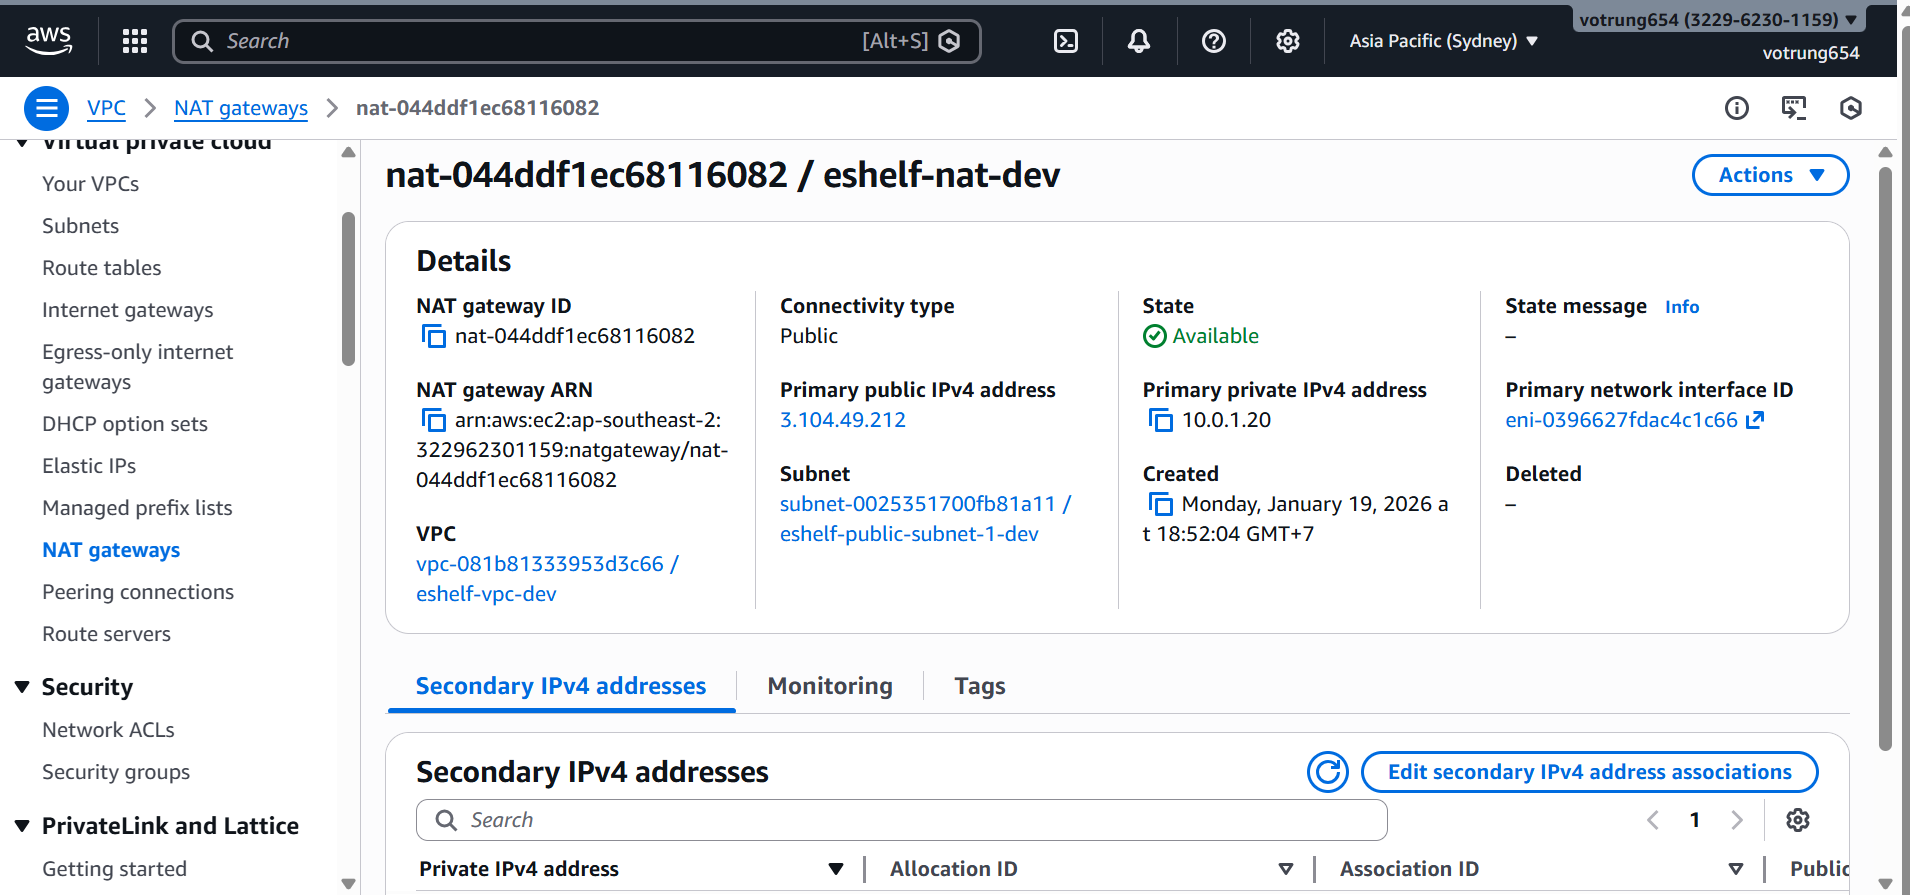
\includegraphics[width=0.9\textwidth]{img/nat_gateway_console.png} 
    \caption{NAT Gateway trạng thái Available và Elastic IP đính kèm}
\end{figure}

\subsection*{3.2 Kiểm thử chức năng NAT (Test Case)}
\textit{(Việc kiểm tra kết nối Internet đã được thực hiện thành công ở TC3 trong Câu 1. Tại đây nhóm xác nhận lại cấu hình EIP).}

% =================================================================
% CÂU 4: EC2 INSTANCES
% =================================================================
\section*{Câu 4: Quản lý máy chủ ảo (EC2 Instances)}
\subsection*{4.1 Cấu hình Instance và phân vai trò}
Hệ thống sử dụng các EC2 Instance với vai trò cụ thể:

\begin{itemize}
    \item \textbf{Bastion Host (Public Instance):}
        \begin{itemize}
            \item \textbf{AMI:} Amazon Linux 2023.
            \item \textbf{Type:} t3.micro.
            \item \textbf{Vai trò:} Điểm truy cập duy nhất (Jump Server) vào hệ thống.
            \item \textbf{Mạng:} Public Subnet. Có địa chỉ Public IP để quản trị viên SSH từ xa.
        \end{itemize}
    \item \textbf{K3s Master \& Workers (Private Instances):}
        \begin{itemize}
            \item \textbf{AMI:} Amazon Linux 2023.
            \item \textbf{Type:} m7i-flex.large (Master), t3.medium (Worker).
            \item \textbf{Vai trò:} Vận hành Kubernetes Cluster (Backend).
            \item \textbf{Mạng:} Private Subnet. Giao tiếp Internet thông qua NAT Gateway.
        \end{itemize}
\end{itemize}
\begin{figure}[H]
    \centering
    % CHỤP ẢNH: Danh sách Instances trên AWS Console (Hiện cột Public IP và Private IP)
    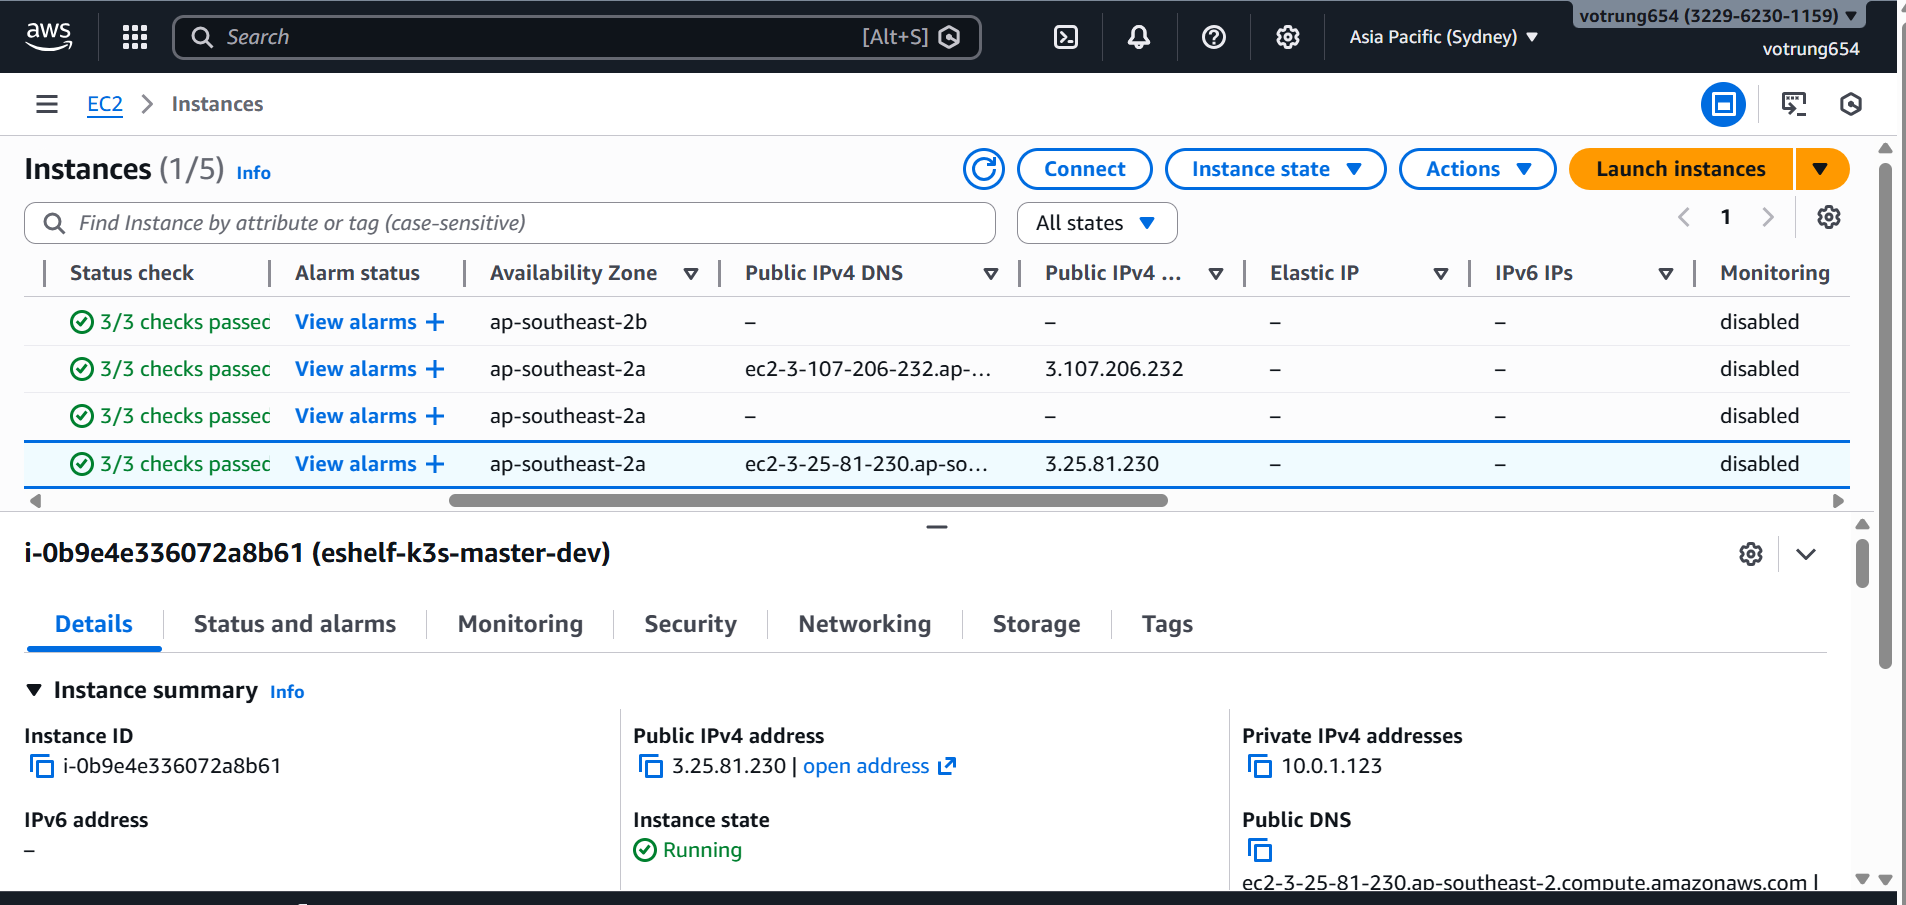
\includegraphics[width=0.9\textwidth]{img/ec2_list.png} 
    \caption{Danh sách EC2 Instances và địa chỉ IP được cấp phát}
\end{figure}
\textbf{ Giải thích kỹ thuật về IP Public của Master Node:} \\
Trong hình trên, máy Master hiển thị có địa chỉ Public IPv4. Đây là tùy chọn được bật tạm thời để phục vụ việc debug nhanh trong môi trường Lab. Tuy nhiên, về mặt bảo mật, Node này vẫn được \textbf{cô lập hoàn toàn} khỏi truy cập từ Internet. Lý do là \textbf{Private Route Table} (đã trình bày ở Câu 2) không có định tuyến inbound từ Internet Gateway, do đó địa chỉ Public IP này không thể truy cập được từ bên ngoài (Unreachable), đảm bảo an toàn tuyệt đối cho hệ thống.
\subsection*{4.2 Kiểm thử truy cập EC2 (Instance Test Cases)}
\begin{table}[H]
    \centering
    \small
    \begin{tabular}{|c|p{4cm}|p{5cm}|p{4cm}|}
        \hline
        \rowcolor{gray!20} \textbf{ID} & \textbf{Mục tiêu kiểm thử} & \textbf{Hành động} & \textbf{Kết quả} \\ \hline
        \textbf{TC5} & \textbf{Isolation Check:} Kiểm tra tính riêng tư của Private Instance & Thử SSH trực tiếp từ máy Local vào Public IP lẫn Private IP của Master Node (\texttt{10.0.1.123}). & \textbf{Connection Timed Out} (Thất bại). Chứng tỏ Instance được cách ly an toàn. \\ \hline
        \textbf{TC6} & \textbf{TC1$\&$TC2:} Public instance có thể truy cập từ Internet, còn Private instance chỉ có thể truy cập từ Public instance. & Lặp lại TC1 và TC2 & Đã thực hiện và đạt được ở TC1 và TC2. \\ \hline
    \end{tabular}
    \caption{Kiểm tra cấu hình và bảo mật Instance}
\end{table}

\begin{figure}[H]
    \centering
    % CHỤP ẢNH MỚI: Cảnh báo Connection Timed Out khi SSH từ local
    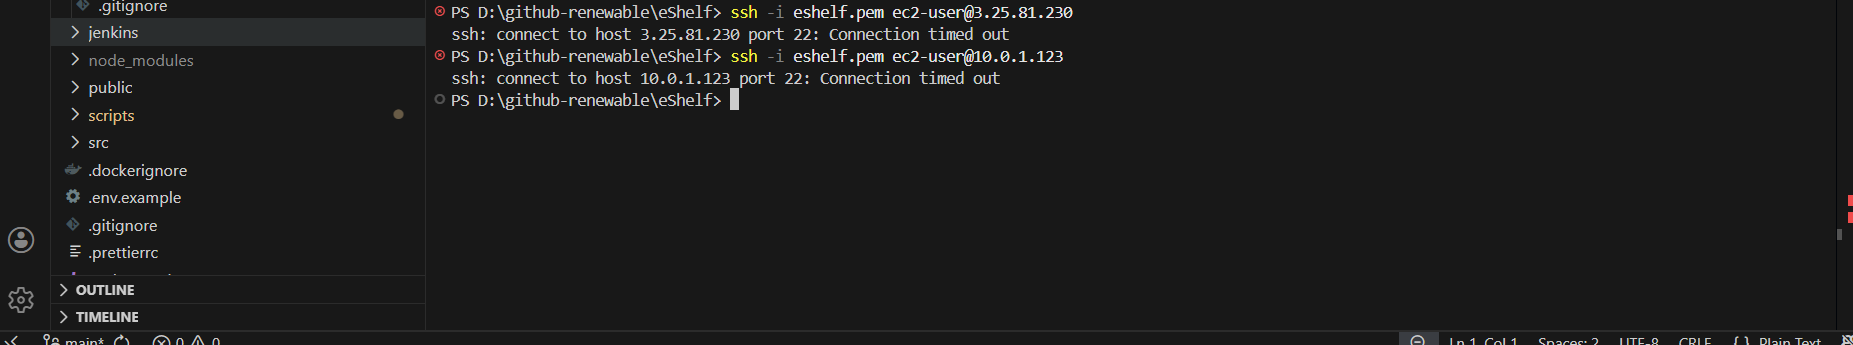
\includegraphics[width=1.0\textwidth]{img/ssh_fail_proof.png} 
    \caption{Kết nối thất bại (Connection time out) khi cố gắng SSH trực tiếp vào Private IP lẫn Public IP của Master tù mấy local (TC5)}
\end{figure}


% =================================================================
% CÂU 5: SECURITY GROUPS
% =================================================================
\section*{Câu 5: Thiết lập Nhóm bảo mật (Security Groups)}
\subsection*{5.1 Cấu hình Tường lửa}
Nhóm đã thiết lập các Security Groups (SG) hoạt động như một tường lửa ảo, kiểm soát chặt chẽ lưu lượng ra vào (Traffic Control) theo mô hình Zero Trust:

\begin{itemize}
    \item \textbf{Bastion Security Group (Public Layer):}
        \begin{itemize}
            \item \textbf{Loại:} Inbound Rule.
            \item \textbf{Cấu hình:} Port 22 (SSH) | Source: \textbf{My IP} (Địa chỉ IP của quản trị viên).
            \item \textbf{Mục đích:} Giới hạn quyền truy cập quản trị, ngăn chặn các cuộc tấn công Brute-force từ Internet.
        \end{itemize}
    \item \textbf{Private Security Group (Application Layer):}
        \begin{itemize}
            \item \textbf{Loại:} Inbound Rule.
            \item \textbf{Cấu hình:} Port 22 (SSH) | Source: \textbf{sg-bastion-id} (Tham chiếu ID của Bastion SG).
            \item \textbf{Mục đích:} Chỉ chấp nhận kết nối SSH từ Bastion Host. Việc sử dụng Reference ID (thay vì IP cứng) giúp rule tự động cập nhật ngay cả khi IP của Bastion thay đổi.
        \end{itemize}
\end{itemize}

\subsubsection*{Minh chứng cấu hình trên AWS Console}

\textbf{1. Cấu hình Bastion SG (Chặn truy cập lạ):}
\begin{figure}[H]
    \centering
    % DÙNG ẢNH BẠN VỪA SỬA LẠI (Chọn My IP thay vì 0.0.0.0/0)
    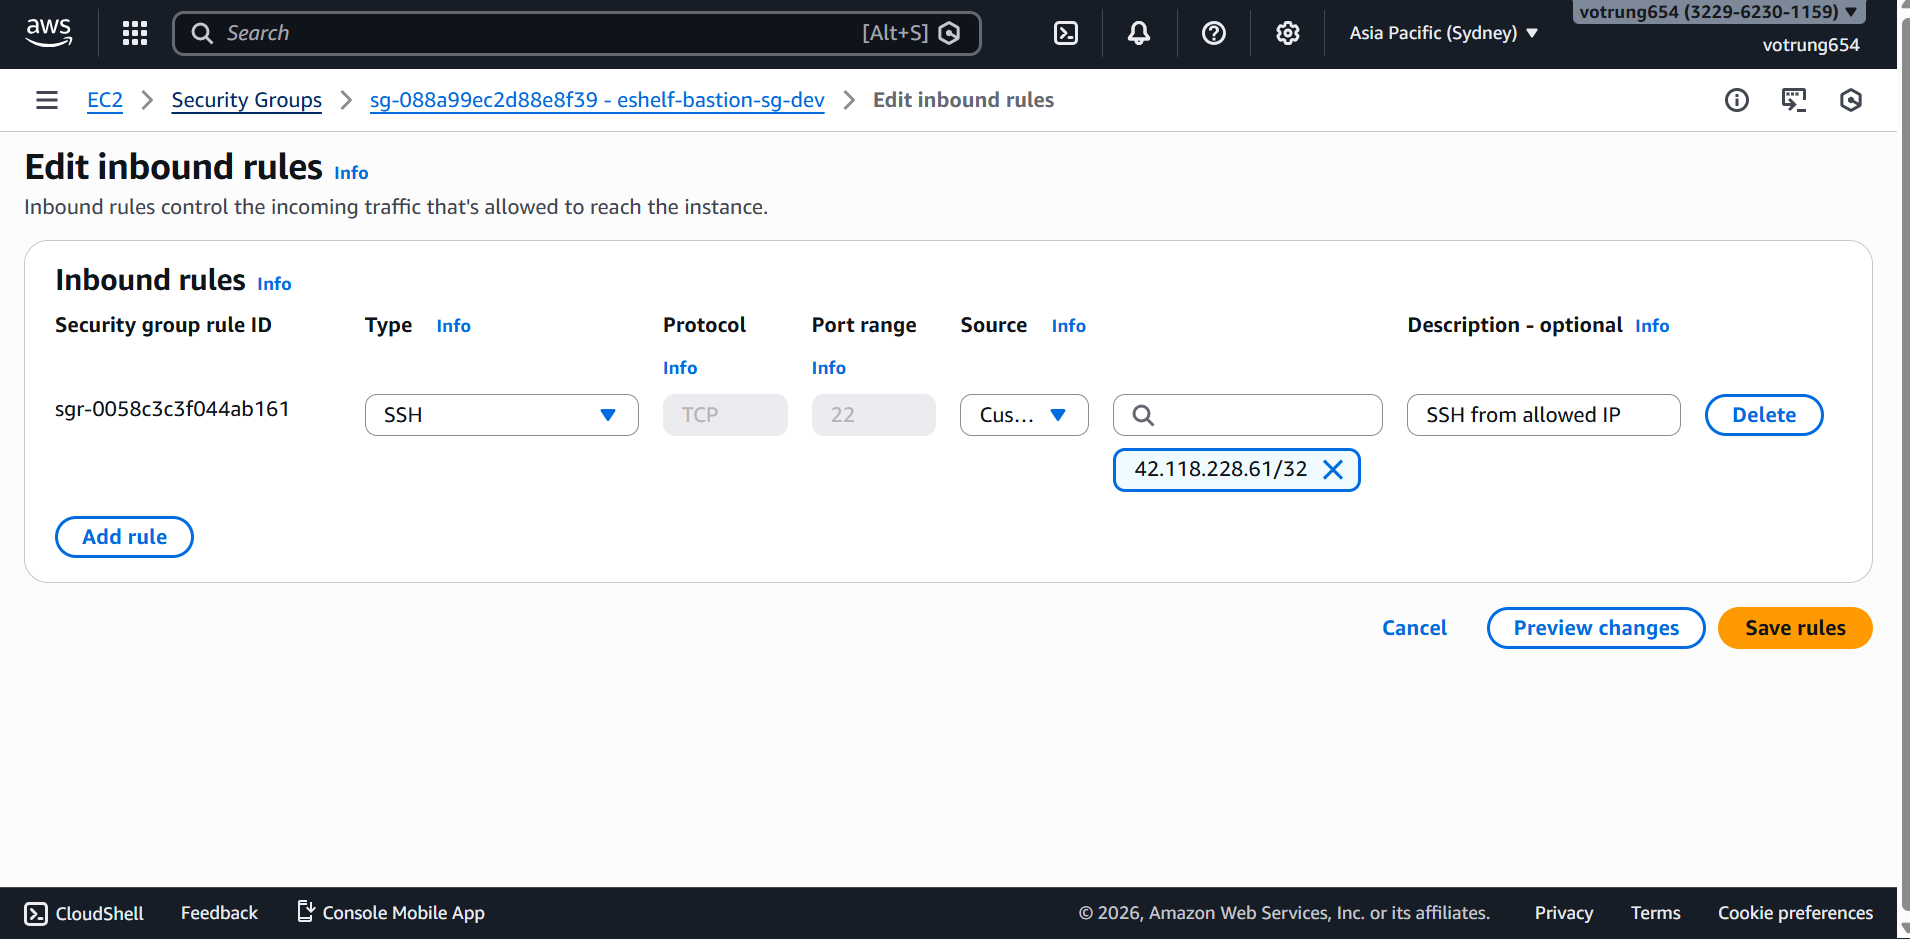
\includegraphics[width=1.0\textwidth]{img/bastion_sg_rules.png} 
    \caption{Bastion SG - Chỉ cho phép SSH từ địa chỉ IP của Developer}
\end{figure}

\textbf{2. Cấu hình Private SG (Reference ID):}
\begin{figure}[H]
    \centering
    % DÙNG ẢNH Private SG (image_9e9d5c.png) BẠN ĐÃ GỬI - ẢNH NÀY RẤT ĐẸP
    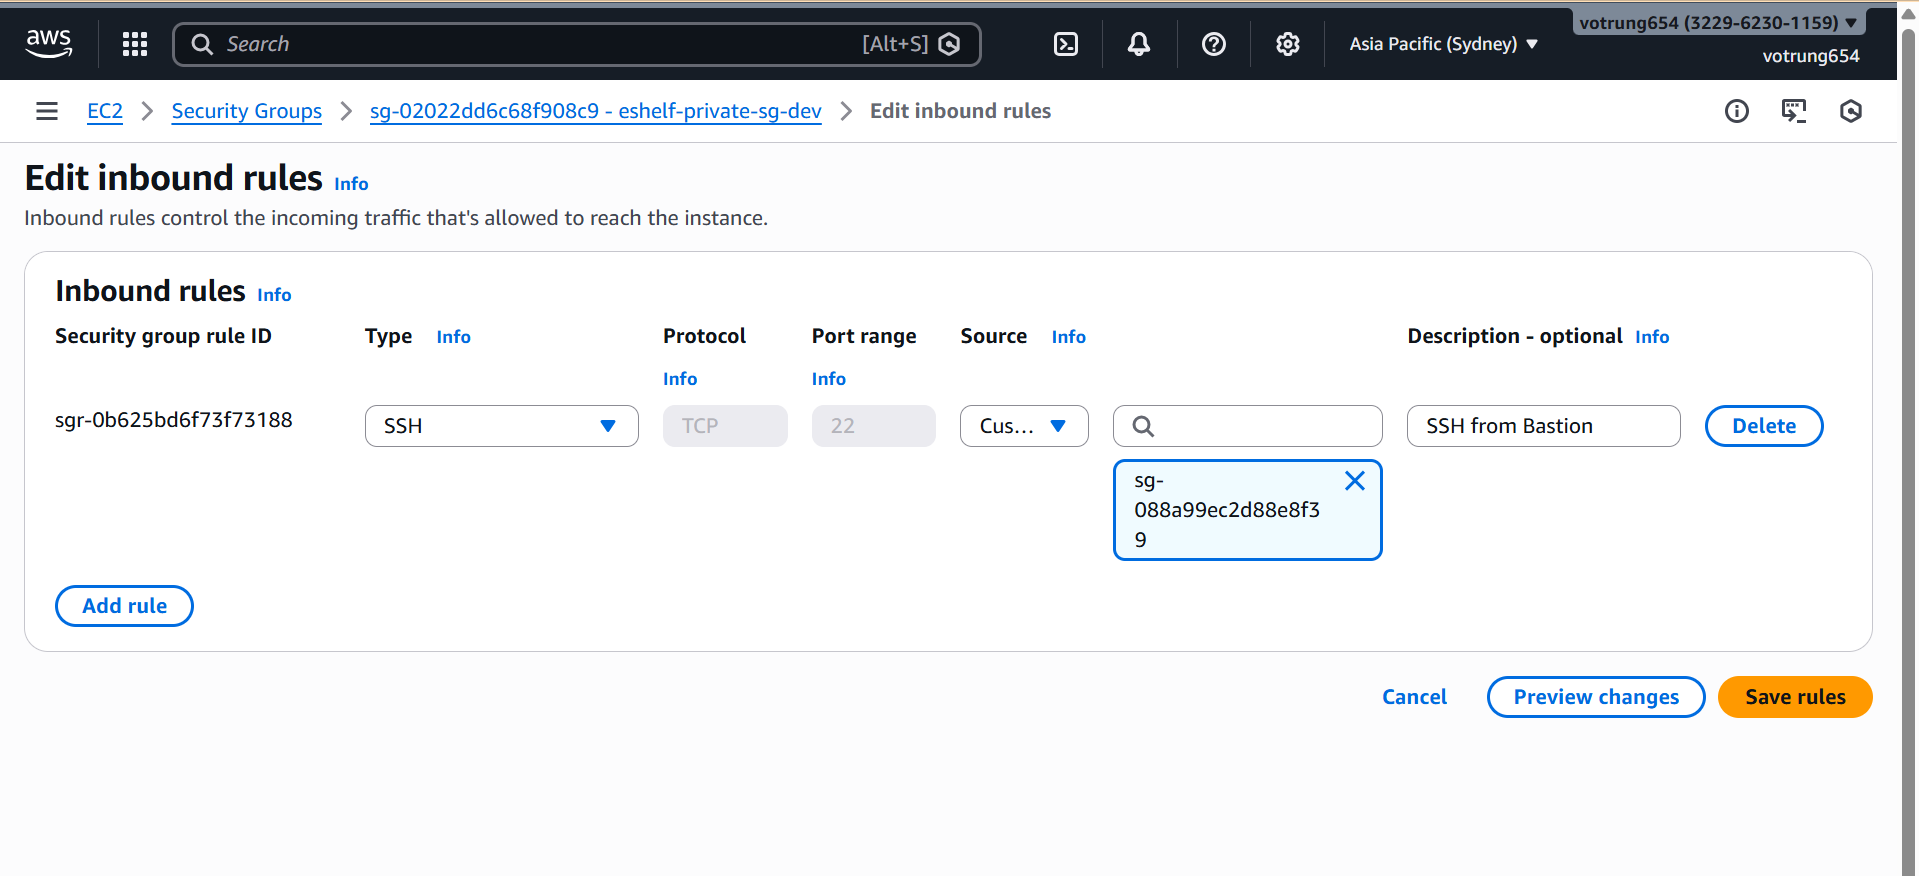
\includegraphics[width=1.0\textwidth]{img/private_sg_rules.png} 
    \caption{Private SG - Source được cấu hình là ID của Bastion SG}
\end{figure}

\subsection*{5.2 Kiểm thử tường lửa (Test Cases)}
Để xác nhận hiệu quả ngăn chặn truy cập trái phép, nhóm thực hiện các kịch bản kiểm thử sau:

\begin{table}[H]
    \centering
    \small
    \begin{tabular}{|c|p{4cm}|p{5cm}|p{4cm}|}
        \hline
        \rowcolor{gray!20} \textbf{ID} & \textbf{Mục tiêu kiểm thử} & \textbf{Hành động} & \textbf{Kết quả} \\ \hline
        \textbf{TC7} & \textbf{Unauthorized Access:} Kiểm tra chặn truy cập trái phép & Thử SSH vào Bastion từ một địa chỉ IP lạ (hoặc dùng VPN đổi IP). & \textbf{Connection Timed Out}. Firewall hoạt động tốt. \\ \hline
        \textbf{TC8} & \textbf{Unauthorized Access:} Kiểm tra chặn truy cập trực tiếp vào Private Instance & Thử SSH từ Local vào Public IP của Master (như đã thực hiện ở TC6). & \textbf{Connection Timed Out}. (Firewall chặn thành công ở TC6). \\ \hline
        \textbf{TC9} & \textbf{Authorized Access:} Kiểm tra luồng truy cập hợp lệ & Từ Bastion Host, thực hiện SSH vào Private IP của Master (\texttt{10.0.1.123}). & \textbf{Connected}. (Giao diện dòng lệnh chuyển sang Master Node, đã thực hiện ở TC2). \\ \hline
    \end{tabular}
    \caption{Kiểm tra hiệu quả của Security Groups}
\end{table}

\subsubsection*{Minh chứng kết quả kiểm thử}
Hình ảnh dưới đây chứng minh hệ thống chỉ cho phép đi theo luồng duy nhất: \textbf{Local $\rightarrow$ Bastion $\rightarrow$ Master}. Mọi nỗ lực truy cập tắt đều bị từ chối.

\begin{figure}[H]
    \centering
    % DÙNG ẢNH SSH JUMP (image_9e21db.png nhưng là phiên bản Timed Out và Connected)
    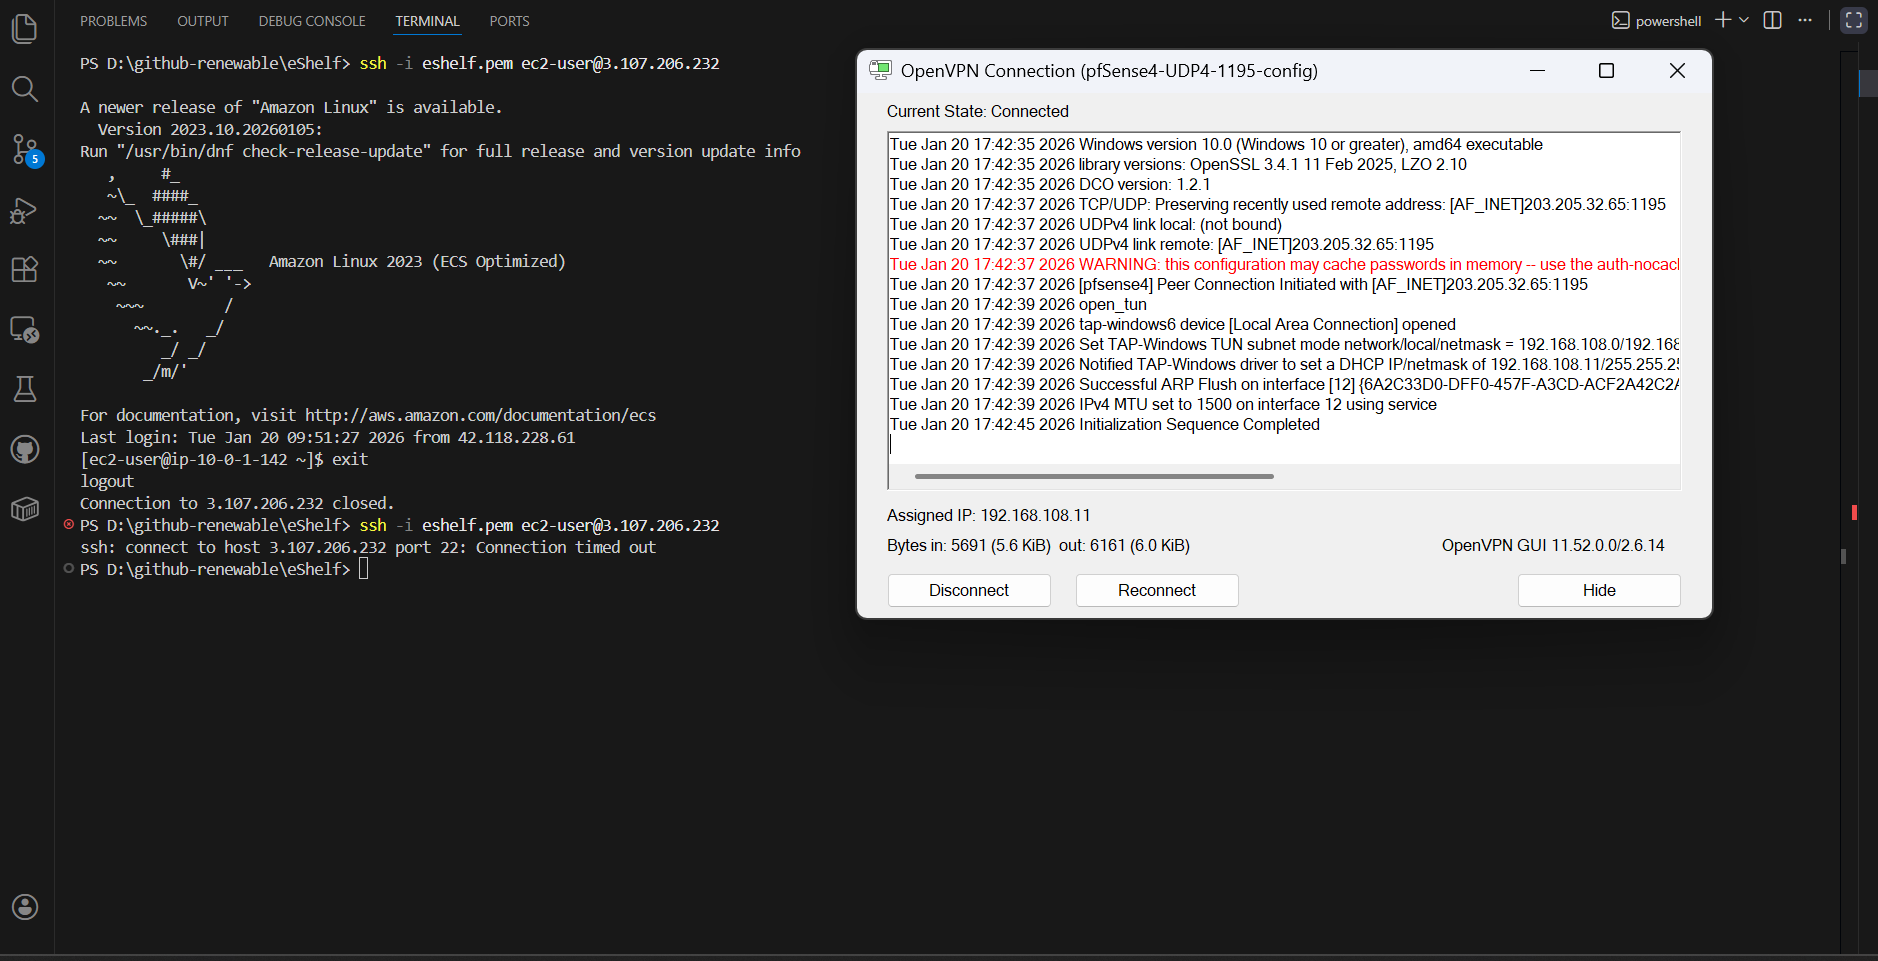
\includegraphics[width=1.0\textwidth]{img/ssh_jump_proof_2.png} 
    \caption{Kiểm thử SSH - Thử SSH vào Bastion từ một địa chỉ IP lạ (VPN của UIT) và thất bại vì không phải IP chuẩn (TC7) trong khi IP chuẩn ở hình 14 thì thành công}
\end{figure}

\section*{Tổng kết}
Bài thực hành đã hoàn thành các yêu cầu đề ra..

\end{document}